%\documentclass[show notes]{beamer}       % print frame + notes

\documentclass[11pt,handout]{beamer}   % only notes
%\documentclass[aspectratio=169]{beamer}              % only frames
\usefonttheme[onlymath]{serif}
\definecolor{DarkGray}{HTML}{63656a}
\setbeamertemplate{note page}[plain]
\setbeamertemplate{navigation symbols}{}
\setbeamertemplate{footline}[text line]{%
    \hfill\strut{\scriptsize\sf\color{DarkGray}\today}\hfill\strut{%
        \scriptsize\sf\color{DarkGray}%
        \quad\insertframenumber/\inserttotalframenumber
    }%
}

\beamertemplatenavigationsymbolsempty


\title[Your Short Title]{Nonlinear Control Systems}
\subtitle{Lsn 2: Phase Plane Analysis}
\author{I. Weintraub, Dr. Cobb, \& Capt. Hess}
\institute{Air Force Institute of Technology}
\date{\today}

\begin{document}

\begin{frame}
  \titlepage
\end{frame}

\begin{frame}
\frametitle{Phase Plane Analysis}
\textbf{What is the Phase Plane?}\\
The Phase plane is a graphical method for studying second order systems.\\
\textbf{Idea:}
In state space, motion trajectories corresponding to various initial conditions, and then to examine the qualitative features of the trajectories\\
\textbf{About Phase Planes}\\
\begin{enumerate}
\item  Graphical method
\item Not restricted to small or smooth nonlinear systems
\end{enumerate}
\end{frame}

\begin{frame}
\frametitle{Phase Plane Analysis}
The Phase plane is used to analyze second order autonomous systems:
\begin{equation}
\begin{aligned}
\dot{x}_1 &= f_1(x_1,x_2)\\
\dot{x}_2 &= f_2(x_1,x_2)
\end{aligned}
\end{equation}
Given a set of initial conditions: $x(0)= x_0$ there exists a solution that defines a trajectory in the phase plane.
\end{frame}

\begin{frame}
\frametitle{Example: Spring Mass System}
%   \framebox{Example}
   \begin{columns}
   \begin{column}{0.5\textwidth}
The dynamics for a Spring-Mass system with no damper:
       \begin{figure}
       
\includegraphics[width=0.5\textwidth]{Figures/Spring_Mass.png}
       \end{figure}
\begin{equation}
\ddot{x}(t) + x = 0
\end{equation}
The state space representation is given by:
\begin{equation}
\begin{aligned}
\dot{x}_1 &= x_2\\
\dot{x}_2 &= -x_1
\end{aligned}
\end{equation}
\end{column}
   \begin{column}{0.5\textwidth}  %%<--- here
       Assuming the system is at rest with initial deflection at length $x_0$, we can see the phase diagram to the right.
\begin{equation}
\begin{aligned}
x(t) &= x_0 \cos (t)\\
\dot{x}(t) &= -x_0 sin(t)
\end{aligned}
\end{equation}
       \begin{center}
       \begin{figure}
       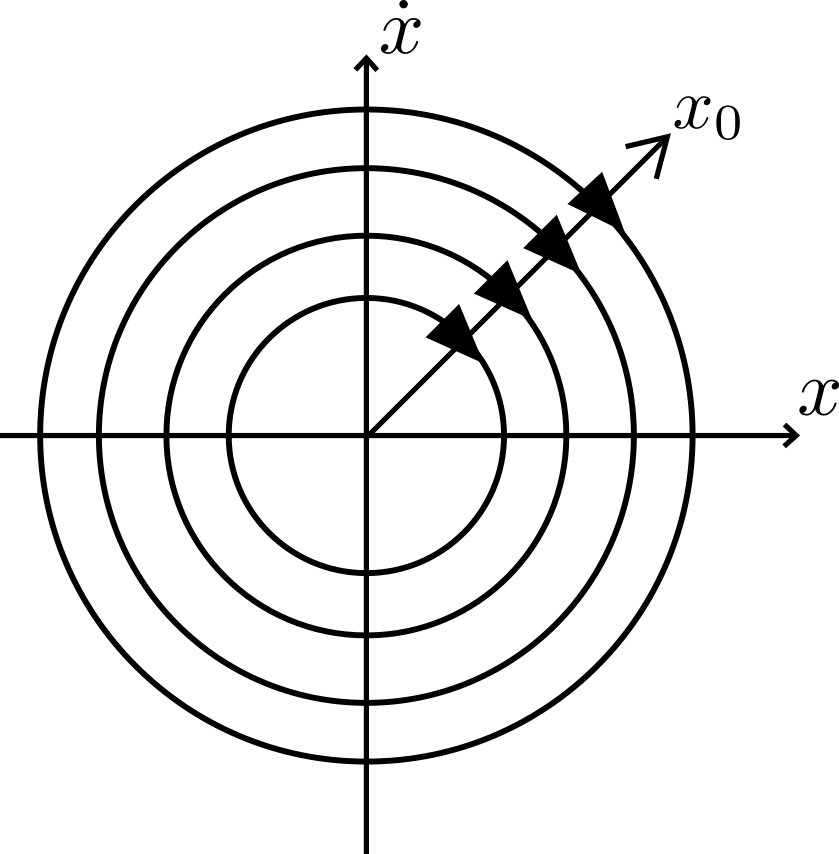
\includegraphics[width=0.5\textwidth]{Figures/Spring_Mass_Phase.png}
       \end{figure}
        \end{center}
   \end{column}
  \end{columns}
\end{frame}

\begin{frame}
\frametitle{Singular and Equilibrium Points}
\begin{itemize}
\item \textbf{Singular Points}: An equilibrium point in the phase plane
\item \textbf{Equilibrium Points} : A point where system dynamics are zero. (e.g.) $\dot{x} = 0$, this implies that $f_1(x_1,x_2) = 0 \;\; \&  \;\; f_2(x_1,x_2) = 0$.
\end{itemize}
\textbf{Note} for a \underline{Linear System} there is usually only one singular point, although in some cases there can be a continuous set of singular points. \\
For Example: $\ddot{x}(t) + \dot{x}(t) = 0$ all points on the real axis are singular points.
\end{frame}

\begin{frame}
\frametitle{1st Order System - Phase Portrait Example}
\begin{columns}
\begin{column}{0.5\textwidth}
Consider:
\begin{equation*}
\dot{x} = -4x+x^3
\end{equation*}
Solving: $-4x+x^3 = 0$
\begin{equation*}
\begin{aligned}
x=-2 &\Rightarrow -4(-2) + (-2)^3 = 0\\
x=2 &\Rightarrow  -4(2) + (2)^3 = 0\\
x=0 &\Rightarrow -4(0) + 0^3 = 0
\end{aligned}
\end{equation*}
\end{column}
\begin{column}{0.5\textwidth}
\begin{centering}
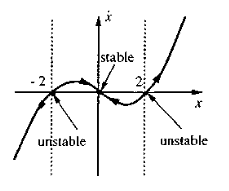
\includegraphics[width=\textwidth]{Figures/Example_3.PNG}
\end{centering}
\textbf{Note:} The direction of the arrows in the figure denote the direction of motion, and whether they point left or right at any particular point is determined by the sign of $\dot{x}$ at that point.
\end{column}
\end{columns}
\end{frame}


\begin{frame}
\frametitle{2nd Order System - Phase Portrait Example}
\begin{columns}
\begin{column}{0.5\textwidth}
Consider:
\begin{equation}
\ddot{x} + 0.6\dot{x}+3x+x^2 = 0
\end{equation}
Converting to State Space:
\begin{equation}
\begin{aligned}
\dot{x}_1 &= x_2\\
\dot{x}_2 &= -0.6x_2-3x_1-x_1^2
\end{aligned}
\end{equation}
The system has two \underline{singular points}: $(0,0)$ and $(-3,0)$.\\The \underline{slope} at any given point in the phase plane can be determined by:
\begin{equation}
\frac{dx_2}{dx_1} = \frac{f_2(x_1,x_2)}{f_1(x_1,x_2)}
\end{equation}
\end{column}
\begin{column}{0.5\textwidth}
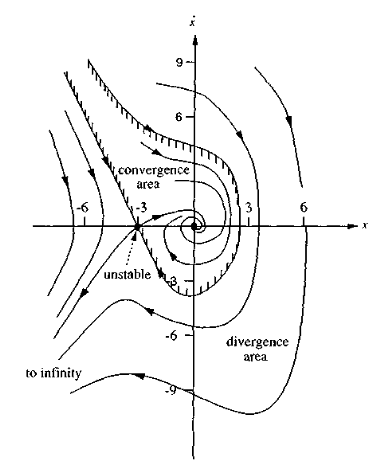
\includegraphics[width=\textwidth]{Figures/Example_2.PNG}
\end{column}
\end{columns}
\end{frame}


\begin{frame}
\frametitle{Constructing Phase Portraits - Analytical Method}
\textbf{Analytical Method}: Using a functional relation between the two phase variables, $x_1$ and $x_2$, in the general form:
\begin{equation*}
g(x_1,x_2,c) = 0
\end{equation*}
Where $c$ represents the effects of initial conditions and external input signals.
\begin{equation*}
x_1(t) = g_1(t) \;\; \& \;\; x_2 = g_2(t)
\end{equation*}
Eliminating the time, $t$, from these equations leads to a generic functional relation in the desired form; for the spring-mass example:
\begin{equation*}
\begin{aligned}
\ddot{x}(t) + x(t) &= 0\\
x^2 + \dot{x}^2 &= x_0^2
\end{aligned}
\end{equation*}
The time is eliminated for the spring-mass example showing that the trajectories lie on a circle with radius $x_0$.
\end{frame}

\begin{frame}
\frametitle{Constructing Phase Portraits}
\small
Another technique eliminates time from the equations through integration. Recall that the slope is given by:
\begin{equation*}
\frac{\frac{dx_2}{dt}}{\frac{dx_1}{dt}} = \frac{dx_2}{dx_1} = \frac{f_2(x_1,x_2)}{f_1(x_1,x_2)}
\end{equation*}
Our Dynamics are:
\begin{equation*}
\ddot{x}+x = 0
\end{equation*}
Using the chain rule:
\begin{equation*}
\ddot{x} = \frac{d\dot{x}}{dx}\frac{dx}{dt}
\end{equation*}
Plugging in and integrating this:
\begin{equation*}
\int \left\lbrace \dot{x} \frac{d\dot{x}}{dx} + x \right\rbrace dx = \int \dot{x}\frac{d\dot{x}}{dx} \; dx + \int x \; dx = 0
\end{equation*}
\begin{equation*}
\left. \frac{\dot{x}^2}{2} \right |_0^x + \left. \frac{x^2}{2} \right |_{x_0}^x = 0 \Rightarrow \frac{\dot{x}^2}{2} + \frac{x^2}{2} - \frac{x_0^2}{2} = 0
\end{equation*}
\begin{equation*}
\dot{x}^2 + x^2 = x_0^2
\end{equation*}
\end{frame}

\begin{frame}
\frametitle{Phase Portrait - Satellite Example}
A rotational unit inertia satellite controlled by a pair of thrusters can either impart a positive or negative thrust to orient the antenna to a desired angle.
\begin{columns}
\begin{column}{0.5\textwidth}
The Control Law:
\begin{equation*}
u(t) =   \left\{
\begin{array}{ll}
      -U &\text{if} \;\; \theta > 0 \\
      U &\text{if} \;\; \theta < 0 \\
      0 & \text{otherwise} \\
\end{array} 
\right.
\end{equation*}\\
\textbf{Case 1} $\theta < 0$ \\
$\ddot{\theta} = U \Rightarrow \dot{\theta}^2 = 2U\theta + \dot{\theta}_0$\\
\textbf{Case 2} $\theta > 0$ \\
$\ddot{\theta} = -U \Rightarrow \dot{\theta}^2 = -2U\theta + \dot{\theta}_0$\\
\textbf{Case 3} $\theta = 0$ \\
$\ddot{\theta} = 0 \Rightarrow \dot{\theta} = \dot{\theta}_0$\\
\end{column}
\begin{column}{0.5\textwidth}
\begin{figure}
\centering
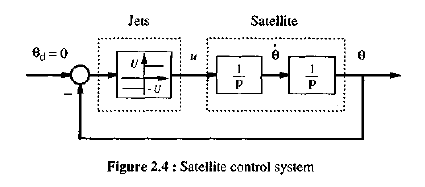
\includegraphics[width=0.9\textwidth]{Figures/Satellite_Control_Block_Diagram.PNG}
\end{figure}
\begin{figure}
\centering
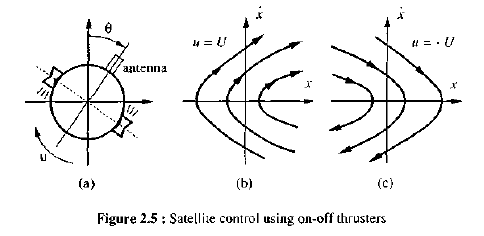
\includegraphics[width=0.9\textwidth]{Figures/Satellite_Phase_1.PNG}
\end{figure}
\end{column}
\end{columns}
\end{frame}

\begin{frame}
\frametitle{Phase Portrait - Satellite Example}
\begin{figure}
\centering
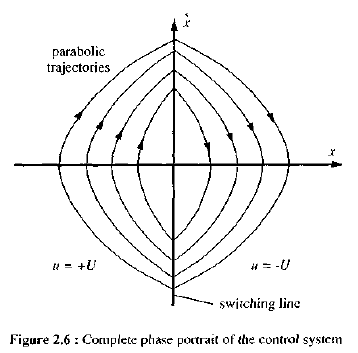
\includegraphics[width=0.7\textwidth]{Figures/Satellite_Phase_2.PNG}
\end{figure}
\end{frame}


\begin{frame}
\frametitle{Constructing Phase Portraits - Method of Isoclines}
Considering the dynamics:
\begin{equation*}
\begin{aligned}
\dot{x}_1 &= f(x_1,x_2)\\
\dot{x}_2 &= f(x_1,x_2)
\end{aligned}
\end{equation*}
The slope of the tangent to the trajectory at $(x_1,x_2)$ is defined by:
\begin{equation*}
\frac{dx_2}{dx_1} = \frac{f_2(x_1,x_2)}{f_1(x_1,x_2)}
\end{equation*}
But for the \textit{method of isoclines} we say that an \underline{isocline} is the locus of the points with a given tangent slope. An isocline with slope, $\alpha$, is defined as:
\begin{equation*}
\frac{dx_2}{dx_1} = \frac{f_2(x_1,x_2)}{f_1(x_1,x_2)} = \alpha \Rightarrow f_2(x_1,x_2) = \alpha f_1(x_1,x_2)
\end{equation*}
\end{frame}

\begin{frame}
\frametitle{Method of Isoclines - Spring Mass}
\begin{columns}
\begin{column}{0.5\textwidth}
\underline{\textbf{Example: Spring-Mass System}}
\begin{equation*}
\ddot{x} + x = 0
\end{equation*}
State Space:
\begin{equation*}
\begin{aligned}
\dot{x}_1 &= x_2\\
\dot{x}_2 &= -x_1
\end{aligned}
\end{equation*}
Isocline:
\begin{equation*}
x_1 + \alpha x_2 = 0
\end{equation*}
\end{column}
\begin{column}{0.5\textwidth}
Phase Portrait:
\begin{figure}
\centering
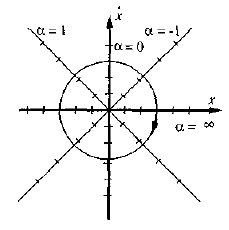
\includegraphics[width=\textwidth]{Figures/Isocline_1.PNG}
\end{figure}
\end{column}
\end{columns}
\end{frame}

\begin{frame}
\frametitle{Method of Isoclines - Van der Pol}
\begin{columns}
\begin{column}{0.5\textwidth}
\underline{\textbf{Example: Van der Pol}}
\begin{equation*}
\ddot{x} + 0.2(x^2-1)\dot{x} + x = 0
\end{equation*}
State Space:
\begin{equation*}
\begin{aligned}
\dot{x}_1 &= x_2\\
\dot{x}_2 &= -0.2(x_1^2-1)x_2 - x_1
\end{aligned}
\end{equation*}
Isocline:
\begin{equation*}
0.2(x_1^2-1)x_2 + x_1 + \alpha x_2 = 0
\end{equation*}
\end{column}
\begin{column}{0.5\textwidth}
Phase Portrait:
\begin{figure}
\centering
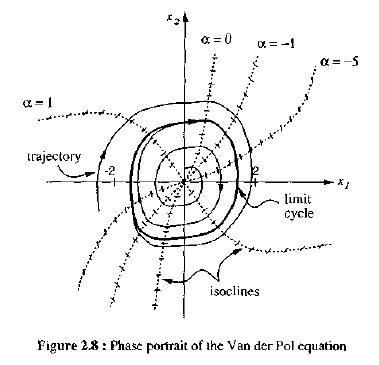
\includegraphics[width=\textwidth]{Figures/Isocline_2.PNG}
\end{figure}
\end{column}
\end{columns}
\end{frame}

\begin{frame}
\frametitle{Phase Plane Analysis of Linear Systems}
\small
\begin{columns}
\begin{column}{0.5\textwidth}
The general form of a linear second-order system is:
\begin{eqnarray}
\label{eq:first}
\dot{x}_1 &= ax_1+bx_2\\
\label{eq:second}
\dot{x}_2 &= cx_1+dx_2
\end{eqnarray}
If we multiply (\ref{eq:second}) by $b$ we obtain:
\begin{equation}
\label{eq:second_b}
b\dot{x}_2 = bcx_1+bdx_2
\end{equation}
Solving (\ref{eq:first}) for $x_2$
\begin{equation}
\label{eq:first_x2}
x_2 = (\dot{x}_1-ax_1)/b
\end{equation}
plugging (\ref{eq:first_x2}) into (\ref{eq:second_b}):
\begin{equation}
\label{eq:bx2}
b\dot{x}_2 = bcx_1+d(\dot{x}_1-ax_1)
\end{equation}
\end{column}
\begin{column}{0.5\textwidth}
If we differentiate (\ref{eq:first}) wrt time:
\begin{equation}
\label{eq:first_time}
\ddot{x}_1 = a\dot{x}_1 + b\dot{x}_2
\end{equation}
plugging (\ref{eq:bx2}) into (\ref{eq:first_time}) we obtain:
\begin{equation}
\begin{aligned}
\ddot{x}_1 &= a\dot{x}_1 + bcx_1+d(\dot{x}_1-ax_1)\\
&= (a+d)\dot{x}_1 + (cb-ad)x_1
\end{aligned}
\end{equation}
Which takes on the form:
\begin{equation}
\label{eq:2ndOrder}
\ddot{x} + A\dot{x} + B x = 0
\end{equation}
To obtain the phase portrait of the linear system, we need to first solve for the time history: (Next Slide)
\end{column}
\end{columns}
\end{frame}

\begin{frame}
\frametitle{Phase Plane Analysis of Linear Systems}
\small
The time history of the solution to the linear system can be identified as:
\begin{eqnarray}
x(t) &= k_1 e^{\lambda_1 t} + k_2 e^{\lambda_2 t} \text{for} \lambda_1 \neq \lambda_2\\
x(t) &= k_1 e^{\lambda_1 t} + k_2 e^{\lambda_1 t} \text{for} \lambda_1 = \lambda_2
\end{eqnarray}
where the eigenvalues $\lambda_1$ and $\lambda_2$ are solutions to the characteristic equation:
\begin{equation}
s^2 + As+B = (s-\lambda_1)(s-\lambda_2) = 0
\end{equation}
Or more explicitly as:
\begin{eqnarray}
\lambda_1 = \frac{-A + \sqrt{A^2 - 4B}}{2}\\
\lambda_2 = \frac{-A - \sqrt{A^2 - 4B}}{2}
\end{eqnarray}
For linear systems described by the second order ODE, (\ref{eq:2ndOrder}), there is only one singular point assuming $B\neq0$, namely the origin. However, the trajectories in the vicinity of this singularity point can display different characteristics.
\end{frame}

\begin{frame}
\frametitle{Phase Plane Analysis of Linear Systems}
\begin{columns}
\begin{column}{0.5\textwidth}
\textbf{Case I : Stable Node}\\
\small{Eigenvalues are Real and Lie in the Left Hand Plane}\\
\textbf{Case II: Unstable Node}\\
\small{Eigenvalues are Real and Lie in the Right Hand Plane}\\
\textbf{Case III: Saddle Point}\\
\small{Eigenvalues are Real and Lie in the Left and Right Hand Planes}\\
\textbf{Case IV: Stable Focus}\\
\small{Eigenvalues are Complex Conjugates and Lie in the Left Hand Plane}\\
\textbf{Case V: Unstable Focus}\\
\small{Eigenvalues are Complex Conjugates and Lie in the Right Hand Plane}\\
\textbf{Case VI: Center Point}\\
\small{Eigenvalues are Purely Imaginary Conjugates}\\
\end{column}
\begin{column}{0.5\textwidth}
\begin{figure}
\centering
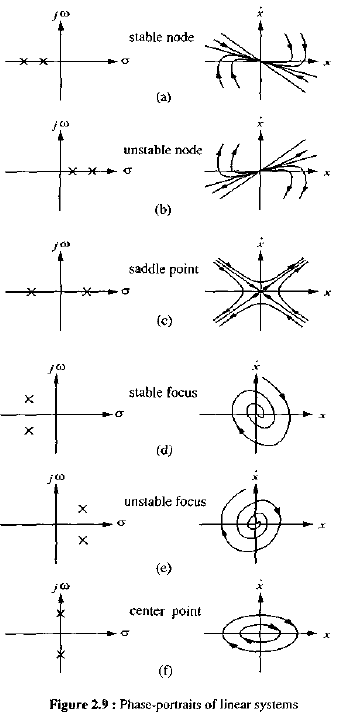
\includegraphics[width=0.7\textwidth]{Figures/Linear_Systems_1.PNG}
\end{figure}
\end{column}
\end{columns}
\end{frame}

\begin{frame}
\frametitle{Limit Cycles}
\small
A \textbf{Limit Cycle} is an isolated closed curve in the phase portrait. The trajectory has to be both closed (indicating periodicity) and isolated (indicating the limiting nature of the cycle).
\begin{enumerate}
\item \textbf{Stable Limit Cycles}: all trajectories in the vicinity converge to the limit cycle as $t \rightarrow \infty$.
\item \textbf{Unstable Limit Cycles}: all trajectories in the vicinity of the limit cycle diverge as $t \rightarrow \infty$.
\item \textbf{Semi-Stable Limit Cycles}: some trajectories in the vicinity of the limit cycle converge, while others diverge as $t \rightarrow \infty$.
\end{enumerate}
\begin{figure}
\centering
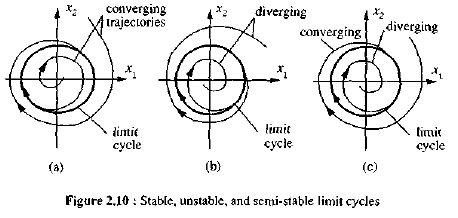
\includegraphics[width=0.7\textwidth]{Figures/Limit_Cycles.PNG}
\end{figure}
\end{frame}

\begin{frame}
\frametitle{Limit Cycles}
\small
\textbf{Existence of Limit Cycles}\\

\begin{enumerate}
\item \textbf{Poincare} Let $N$ be the number of nodes, centers, and foci enclosed by a limit cycle. Let $S$ be the number of enclosed saddle points. If a limit cycle exists in the second-order autonomous system, then $N=S+1$. \underline{Basically a limit cycle must contain least one equilibrium point}
\item \textbf{Poincare - Bendixson} If a trajectory of the second-order autonomous system remains in a finite region $\Omega$, then one of the following is true:
\begin{enumerate}
\item the trajectory goes to an equilibrium point
\item the trajectory tends to an asymptotically stable limit cycle
\item the trajectory is itself a limit cycle
\end{enumerate}
\item \textbf{Bendixson} For a nonlinear system, no limit cycle can exist in a region $\Omega$ of the phase plane in which $\partial f_1 / \partial x_1 + \partial f_2 / \partial x_2$ does not vanish and does not change sign. (example on next slide)
\end{enumerate}
\end{frame}

\begin{frame}
\frametitle{Limit Cycles}
\small
\begin{columns}
\begin{column}{0.5\textwidth}
\textbf{Poincare Example}:
Nodes: $N = 1$, Saddles: $S=0$\\
$N=S+1$ holds
\begin{figure}
\centering
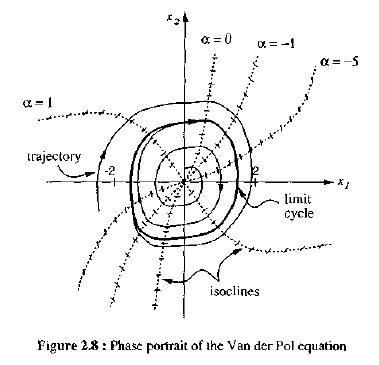
\includegraphics[width=1.0\textwidth]{Figures/Isocline_2.PNG}
\end{figure}
\end{column}
\begin{column}{0.5\textwidth}
\textbf{Bendixon Example}
\begin{eqnarray*}
\dot{x}_1 = g(x_2) + 4x_1x_2^2\\
\dot{x}_2 = h(x_1) + 4x_1^2x_2
\end{eqnarray*}
Since
\begin{equation*}
\frac{\partial f_1}{\partial x_1} + \frac{\partial f_2}{\partial x_2} = 4(x_1^2+x_2^2) 
\end{equation*}
Which is always strictly positive (except at the origin), the system does not contain a limit cycle anywhere in the phase plane.
\end{column}
\end{columns}
\end{frame}

\begin{frame}
\frametitle{Exercise 1: Phase Portrait}
\small 
\textbf{Draw the phase portrait and discuss the properties of the linear, unity feedback control system of open-loop transfer function}
\begin{equation*}
G(s) = \frac{10}{s(1+0.1s)} \Rightarrow G(s) = \frac{100}{(s)(s+10)} \Rightarrow 100X(s) = (s^2 + 10s + 0 ) Y(S)
\end{equation*}
Using the connonical form:
\begin{equation*}
\begin{bmatrix}
\dot{x}_1\\ \dot{x}_2
\end{bmatrix} = 
\begin{bmatrix}
-10 & 0\\ 1 & 0
\end{bmatrix} \begin{bmatrix}
x_1 \\ x_2
\end{bmatrix} \Rightarrow 
\begin{aligned}
\dot{x}_1 &= -10 x_1 \\ \dot{x}_2 &= x_1
\end{aligned}
\end{equation*}
From the denominator of the factored transfer function we have eigen values located at $-10$ and $0$.\\
\begin{columns}
\begin{column}{0.5\textwidth}
\centering
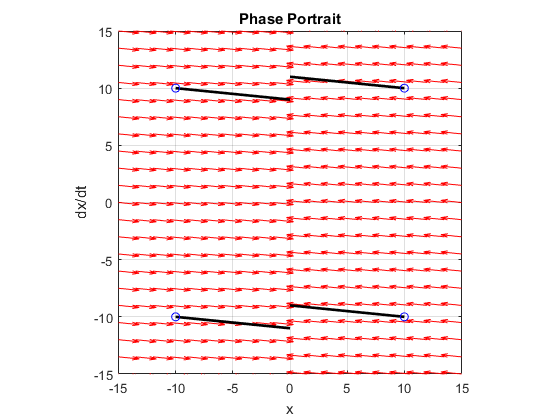
\includegraphics[width = \textwidth]{Figures/Exersize21.png}
\end{column}
\begin{column}{0.5\textwidth}
\small
The open loop transfer function has a single pole on the Real-Imaginary Axis and one in the Left Hand Plane. The Phase Portrait shows that if the system tends toward the vertical $\dot{x}$ line.
\end{column}
\end{columns}

% \begin{figure}
% \centering
% 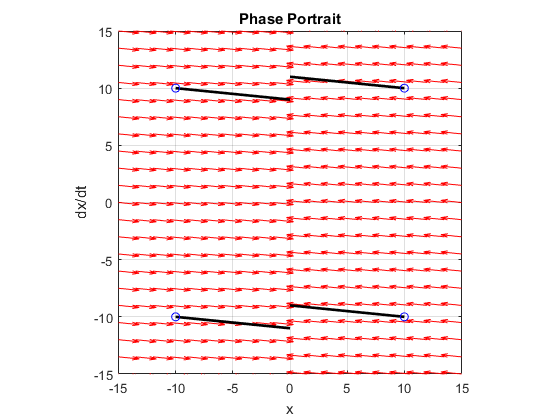
\includegraphics[width = 0.4\textwidth]{Figures/Exersize21.png}
% \end{figure}
\end{frame}

\begin{frame}
\frametitle{Exercise 2: Isoclines}
\begin{columns}
\begin{column}{0.5\textwidth}
\small
\textbf{Draw the phase portrait of the following systems using isoclines:}
\begin{equation*}
\ddot{\theta} + \dot{\theta} + 0.5\theta = 0
\end{equation*}
Using State Space:
\begin{equation*}
x_1 = \theta \;\; \& \;\; x_2 = \dot{\theta}
\end{equation*}
The Second Order ODE becomes:
\begin{equation*}
\begin{aligned}
\dot{x_1} = x_2\\
\dot{x_2} = -x_2 - 0.5 x_1
\end{aligned}
\end{equation*}
Using the Method of Isoclines:
\begin{equation*}
\frac{dx_2}{dx_1} = \frac{-x_2 - 0.5 x_1}{x_2} = \alpha
\end{equation*}
\end{column}
\begin{column}{0.5\textwidth}
\small
\centering
$\alpha = 1 \Rightarrow \dot{\theta} = -0.25 \theta$\\
$\alpha = 0 \Rightarrow \dot{\theta} = -0.5 \theta$\\
$\alpha = -1 \Rightarrow \theta = 0$
\begin{figure}
\centering
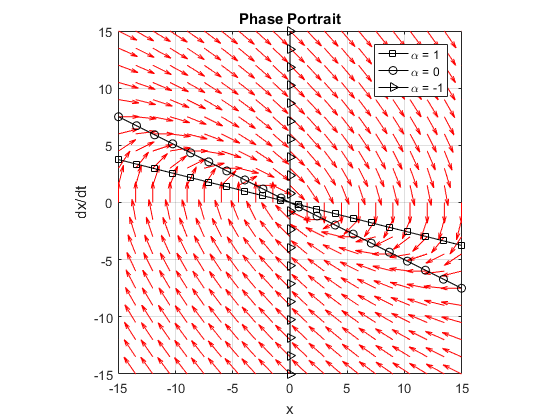
\includegraphics[width = \textwidth]{Figures/Isocline_3.png}
\end{figure}
\end{column}
\end{columns}
\end{frame}

\begin{frame}
\frametitle{Exercise 3: Bendixson}
\begin{columns}
\begin{column}{0.5\textwidth}
\small
\textbf{Van der Pol Equation:}
\begin{equation*}
\ddot{x} + 0.2(x^2 - 1)\dot{x}+x = 0
\end{equation*}
In State Space:
\begin{equation*}
\begin{aligned}
\dot{x}_1 &= x_2\\
\dot{x}_2 &= -0.2(x_1^2 - 1)x_2 - x_1
\end{aligned}
\end{equation*}
Computing required partials for Bendixson:
\begin{equation*}
\frac{\partial f_1}{\partial x_1} = 0 \;\; \& \;\; \frac{\partial f_2}{x_2} = -0.2(x_1^2-1)
\end{equation*}
We find that the summation of the partials is negative define and therefore a limit cycle may exist in the phase plane.
\end{column}
\begin{column}{0.5\textwidth}
\centering
\textbf{Van der Pol Phase Portrait}
\begin{figure}
\centering
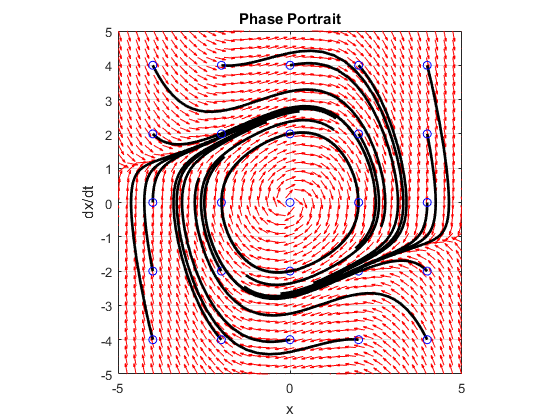
\includegraphics[width = \textwidth]{Figures/VanderPol.png}
\end{figure}
\end{column}
\end{columns}
\end{frame}

%%
%% Blank Slide
%%
% \begin{frame}
% \frametitle{}
% \end{frame}

%%
%% Dual Column Slide
%%
% \begin{frame}
% \frametitle{1st Order System - Phase Plane Example}
% \begin{columns}
% \begin{column}{0.5\textwidth}
% Text 1
% \end{column}
% \begin{column}{0.5\textwidth}
% Text 2
% \end{column}
% \end{columns}
% \end{frame}






\end{document}